\section{Methodology}
\begin{wrapfigure}{r}{0.48\textwidth}
   \begin{center}
   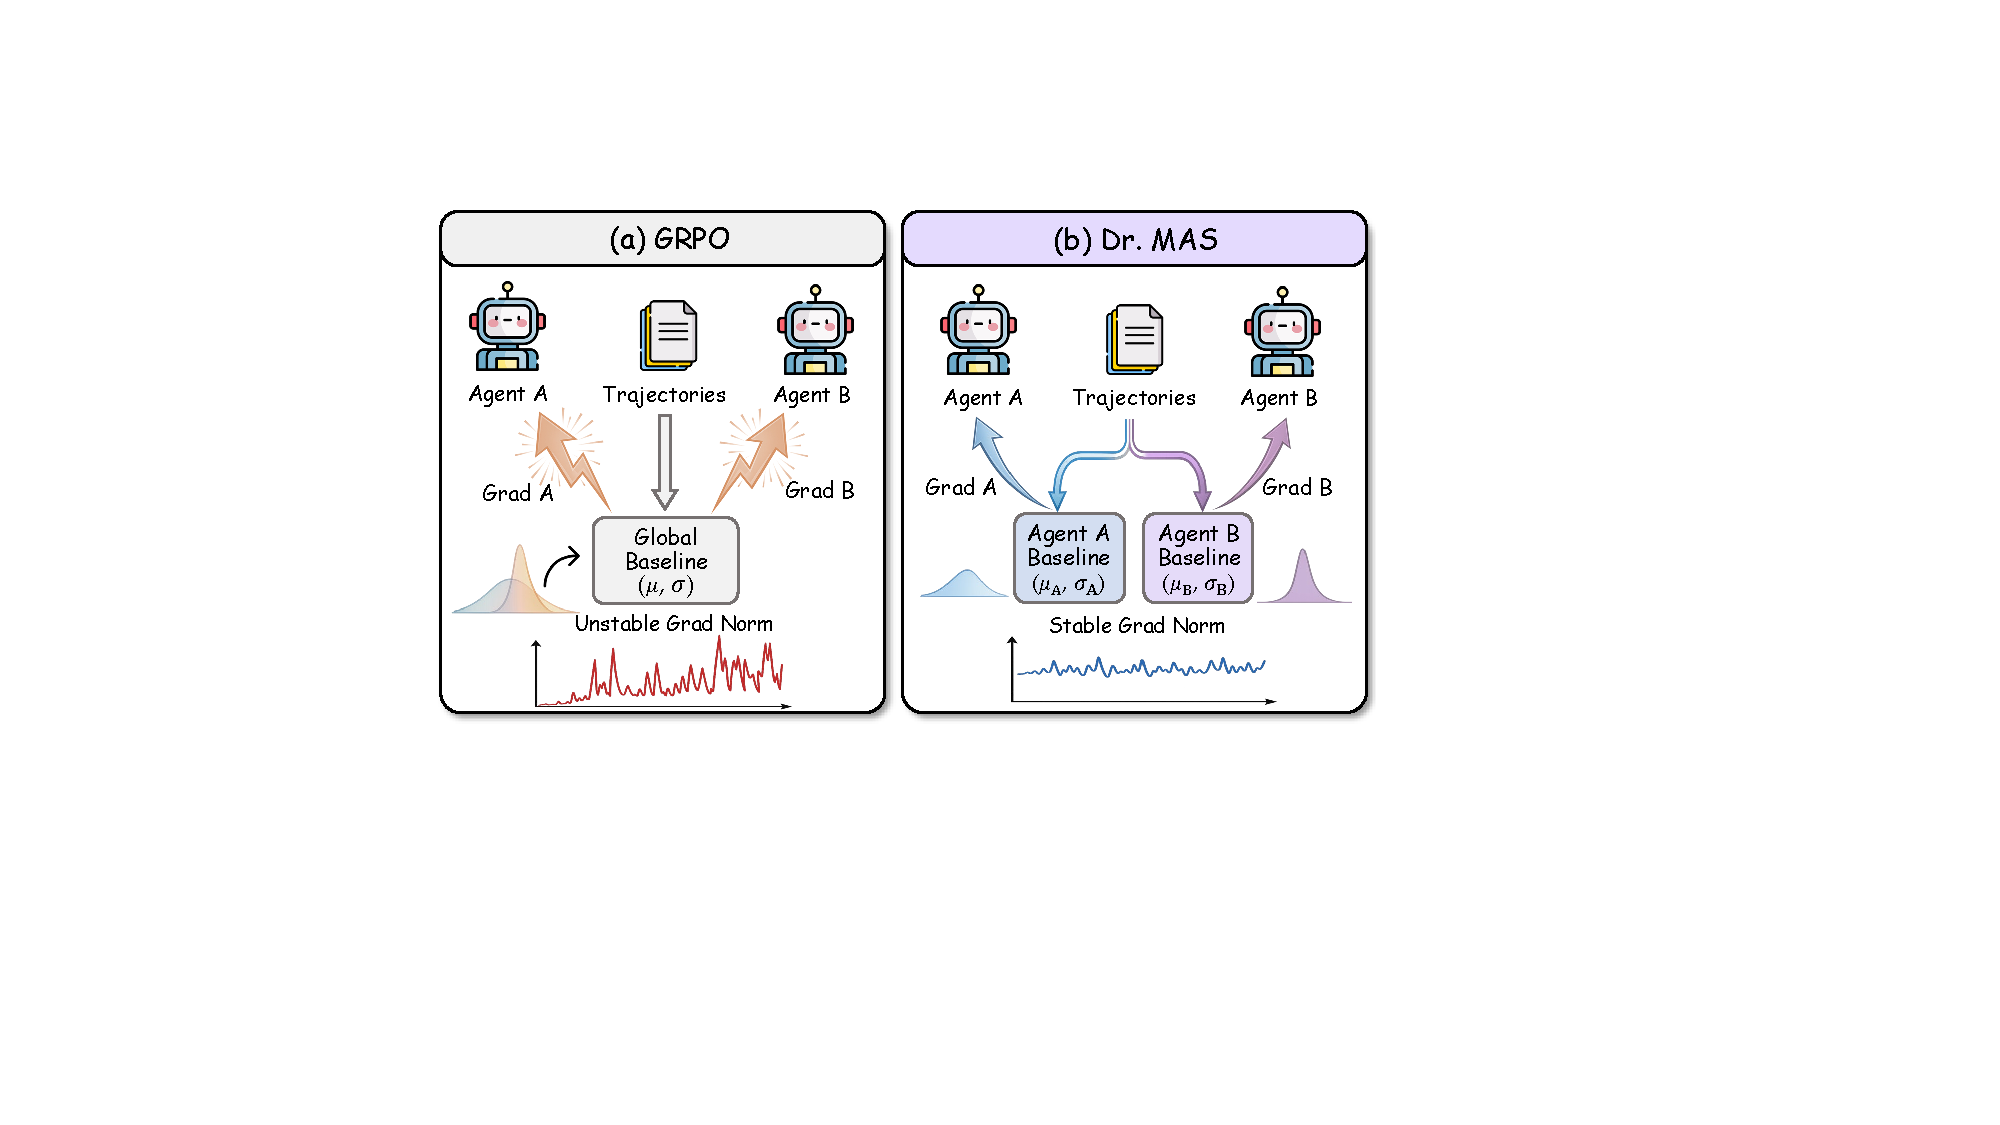
\includegraphics[width=1\linewidth]{./figure/method_comparison.pdf}
   \end{center}
   \vspace{-0.1in}
   \caption{Algorithm comparison. (a) GRPO with global baseline $(\mu,\sigma)$ can cause unstable gradient norm. (b) \methodname{} with per-agent normalization $(\mu_k,\sigma_k)$ stabilizes the training of MAS.}
   \label{fig:method_comparison}
   \vspace{-0.1in}
\end{wrapfigure}
In a multi-agent LLM system, different agents often specialize in
distinct functions (e.g., information retrieval vs. answer synthesis, high-level planning vs. low-level execution), and consequently can exhibit substantially different reward distributions. We find that using vanilla GRPO with the global baseline $(\mu,\sigma)$ for all agents can be suboptimal: some agents may consistently operate in reward distributions above the global mean, while others remain below it. This persistent bias in how advantages are normalized can introduce a deterministic shift in the effective advantages seen by each agent, which in turn can inflate gradient-estimator variance and destabilize training.

In this section, we introduce \methodname{} by (\textbf{1}) theoretically formalizing the instability and analyzing the second moment of the per-agent gradient under GRPO optimization (Section~\ref{sec:risk}); (\textbf{2}) proposing an agent-wise remedy that calibrates each agent's advantage using its own reward statistics, thereby improve the training stability (Section~\ref{sec:remedy}); and (\textbf{3}) describing a system framework that implements efficient end-to-end RL training recipe for multi-agent LLM systems (Section~\ref{sec:framework}). The complete pseudo code of \methodname{} is provided in Appendix~\ref{app:pseudocode}.


\subsection{Risk of Gradient Norm Explosion}
\label{sec:risk}
To focus on how advantage normalization causes the instability in MAS training, we perform a theoretical analysis of the gradient norm. We base our analysis on the unclipped GRPO gradient (clipping and other regularization only further bound the update and are orthogonal to the gradient issue we study).
For each agent $k$, and for each step $(i,t)$ such that $k_t^i = k$, we define
the \emph{score function} as $z_{i,t}^{(k)} \triangleq \nabla_{\theta_k} \rho_{\theta_k}(\bm{a}_t^{i})$ and corresponding (unclipped) GRPO gradient contribution as
\begin{equation}
    \tilde{g}_k^{\mathrm{global}}
    \triangleq
    \frac{R^i - \mu}{\sigma}\,
    z_{i,t}^{(k)}.
\end{equation}
Here, $(\mu,\sigma)$ are the mean and standard deviation used by vanilla GRPO. We assume that each agent’s score function has a bounded second moment:
\begin{assumption}
\label{assump:score}
\emph{For each agent $k$, there exists a constant $C_k < \infty$ such that $\mathbb{E}\big[\,\|z_{i,t}^{(k)}\|^2\,\big] \le C_k$.}
\end{assumption}
Then we can express the second moment of the per-agent gradient as follows.
\begin{lemma}
\label{lem:global-second-moment}
Under Assumptions~\ref{assump:score}, for any agent $k$,
\begin{equation}
\nonumber
\mathbb{E}_{\bm{a}_t^i\sim \mathcal{Y}_k}\big[\|\tilde{g}_k^{\mathrm{global}}\|^2\big]
{=} \mathbb{E}_{\bm{a}_t^i\sim \mathcal{Y}_k}\big[\|z_{i,t}^{(k)}\|^2\big]\,
  \frac{\sigma_k^2 + (\mu_k - \mu)^2}{\sigma^2} + \Delta_k,
\end{equation}
where $\mu_k \triangleq \frac{1}{|\mathcal{Y}_k|}\sum_{\bm{a}_t^i\in \mathcal{Y}_k} R^i$, $\sigma_k^2 \triangleq \frac{1}{|\mathcal{Y}_k|}\sum_{\bm{a}_t^i\in \mathcal{Y}_k} (R^i - \mu_k)^2$
are the mean and variance when sampling
time steps uniformly from $\mathcal{Y}_k$ (i.e., when agent $k$ is active). $\Delta_k$ is a score-reward covariance correction term.
\end{lemma}
See Appendix~\ref{app:proof_lemma_global_second_moment} for the proof.
Lemma~\ref{lem:global-second-moment} separates the per-agent gradient norm into a dominant scaling factor and a residual covariance correction. The multiplicative factor $\bigl(\sigma_k^2+(\mu_k-\mu)^2\bigr)/\sigma^2$ grows when agent $k$ operates in a reward distribution whose mean is far from the global mean or agent $k$’s conditional reward variance is much larger than the global variance.
The term $\Delta_k$ captures the residual score-reward correlation. In large-scale LLM training, rewards are typically low-dimensional signals of final task quality (e.g., pass/fail for reasoning, correctness for coding), while $z_{i,t}^{(k)}$ depends mainly on the local token-level stochasticity of the policy. Empirically, their covariance is often much smaller than the dominant scaling factor $\mathbb{E}_k[\|z_{i,t}^{(k)}\|^2](\sigma_k^2 + (\mu_k - \mu)^2)/\sigma^2$. This decomposition reveals the intrinsic instability of global normalization of GRPO in heterogeneous multi-agent training: a large deviation in the dominant scaling factor can inflate the gradient and lead to unstable updates. We formalize this phenomenon below.
\begin{proposition}[Gradient-Norm Inflation]
\label{prop:gradient-inflation}
As either the normalized mean deviation
$|\mu_k - \mu| / \sigma$ or the normalized variance ratio
$\sigma_k^2 / \sigma^2$ becomes large, the second moment of
$\tilde{g}_k^{\mathrm{global}}$ grows at least linearly. Consequently, along any training process for which there exists a sequence of iterations indexed by $m$ such that
$$
\frac{\sigma_{k,m}^2 + (\mu_{k,m} - \mu_m)^2}{\sigma_m^2} \to \infty, \quad  \mathbb{E}\bigl[\|\tilde{g}_m^{\mathrm{global}}\|^2\bigr] \to \infty,
$$
where $\tilde{g}_{m}^{\mathrm{global}} = (\tilde{g}_{1,m}^{\mathrm{global}},\dots,\tilde{g}_{K,m}^{\mathrm{global}})$ stacking all LLM agents' gradients.
\end{proposition}
The proof is provided in Appendix~\ref{app:proof_prop_gradient_inflation}. Proposition~\ref{prop:gradient-inflation} demonstrates that gradient-norm inflation can be triggered by \emph{any} agent whose reward distribution is poorly aligned with the global baseline. In practice, the gradient norms in such cases typically do not reach mathematical infinity. However, they often grow large enough and trigger severe gradient spikes, thus destabilizing the training process of the entire multi-agent LLM system.


\subsection{Agent-Wise Remedy}
\label{sec:remedy}
Fortunately, Proposition~\ref{prop:gradient-inflation} suggests a straightforward and effective remedy: calibrating each agent’s advantages using reward statistics computed exclusively on the steps where that agent is active.
Specifically, we replace the global baseline $(\mu,\sigma)$ with $(\mu_k,\sigma_k)$, which ensures that $(\sigma_k^2 + (\mu_k - \mu)^2)/\sigma^2=1$. In practice, this corresponds to normalizing each agent’s reward using its own empirical mean and variance: 
% \begin{equation}
%     A^{i,k}_{\mathrm{agent}} = \frac{R^i - \mu_k}{\sigma_k}, 
%     \qquad 
%     \mu_k \triangleq \frac{1}{|\mathcal{Y}_k|}
%     \sum_{\bm{a}_t^i\in \mathcal{Y}_k} R^i,
%     \qquad
%     \sigma_k^2 \triangleq \frac{1}{|\mathcal{Y}_k|}
%     \sum_{\bm{a}_t^i\in \mathcal{Y}_k} (R^i - \mu_k)^2
% \end{equation}
\begin{equation}
    A^{i,k}_{\mathrm{agent}} = \frac{R^i - \mu_k}{\sigma_k},
\end{equation}
where $\mu_k \triangleq \frac{1}{|\mathcal{Y}_k|}\sum_{\bm{a}_t^i\in \mathcal{Y}_k} R^i$ and $\sigma_k^2 \triangleq \frac{1}{|\mathcal{Y}_k|}\sum_{\bm{a}_t^i\in \mathcal{Y}_k} (R^i - \mu_k)^2$. Therefore, an analysis analogous to
Lemma~\ref{lem:global-second-moment} yields
\begin{equation}
    \mathbb{E}_{\bm{a}_t^i\sim \mathcal{Y}_k}\bigl[\|\tilde{g}_k^{\mathrm{agent}}\|^2\bigr]=\mathbb{E}_{\bm{a}_t^i\sim \mathcal{Y}_k}\bigl[\|z_{i,t}^{(k)}\|^2\bigr] +\Delta_k,
\end{equation}
where $\tilde{g}_k^{\mathrm{agent}}=\frac{R^i - \mu_k}{\sigma_k}\, z_{i,t}^{(k)}$. Thus, under agent-wise normalization, the second moment of each agent’s gradient is bounded purely by its own score statistics. Crucially, this effect is inherently \emph{multi-agent}: as the number of specialized agents increases and their roles become more heterogeneous, a single global baseline is increasingly likely to be badly aligned with some agents, leading to gradient norm explosion. As shown in Figure~\ref{fig:method_comparison}, a simple agent-wise remedy, by adapting to each agent’s own statistics, achieves keeping all gradients in a comparable, well-conditioned range, while still enabling cooperative optimization of the overall multi-agent LLM system.

\begin{figure*}[t]
   \begin{center}
   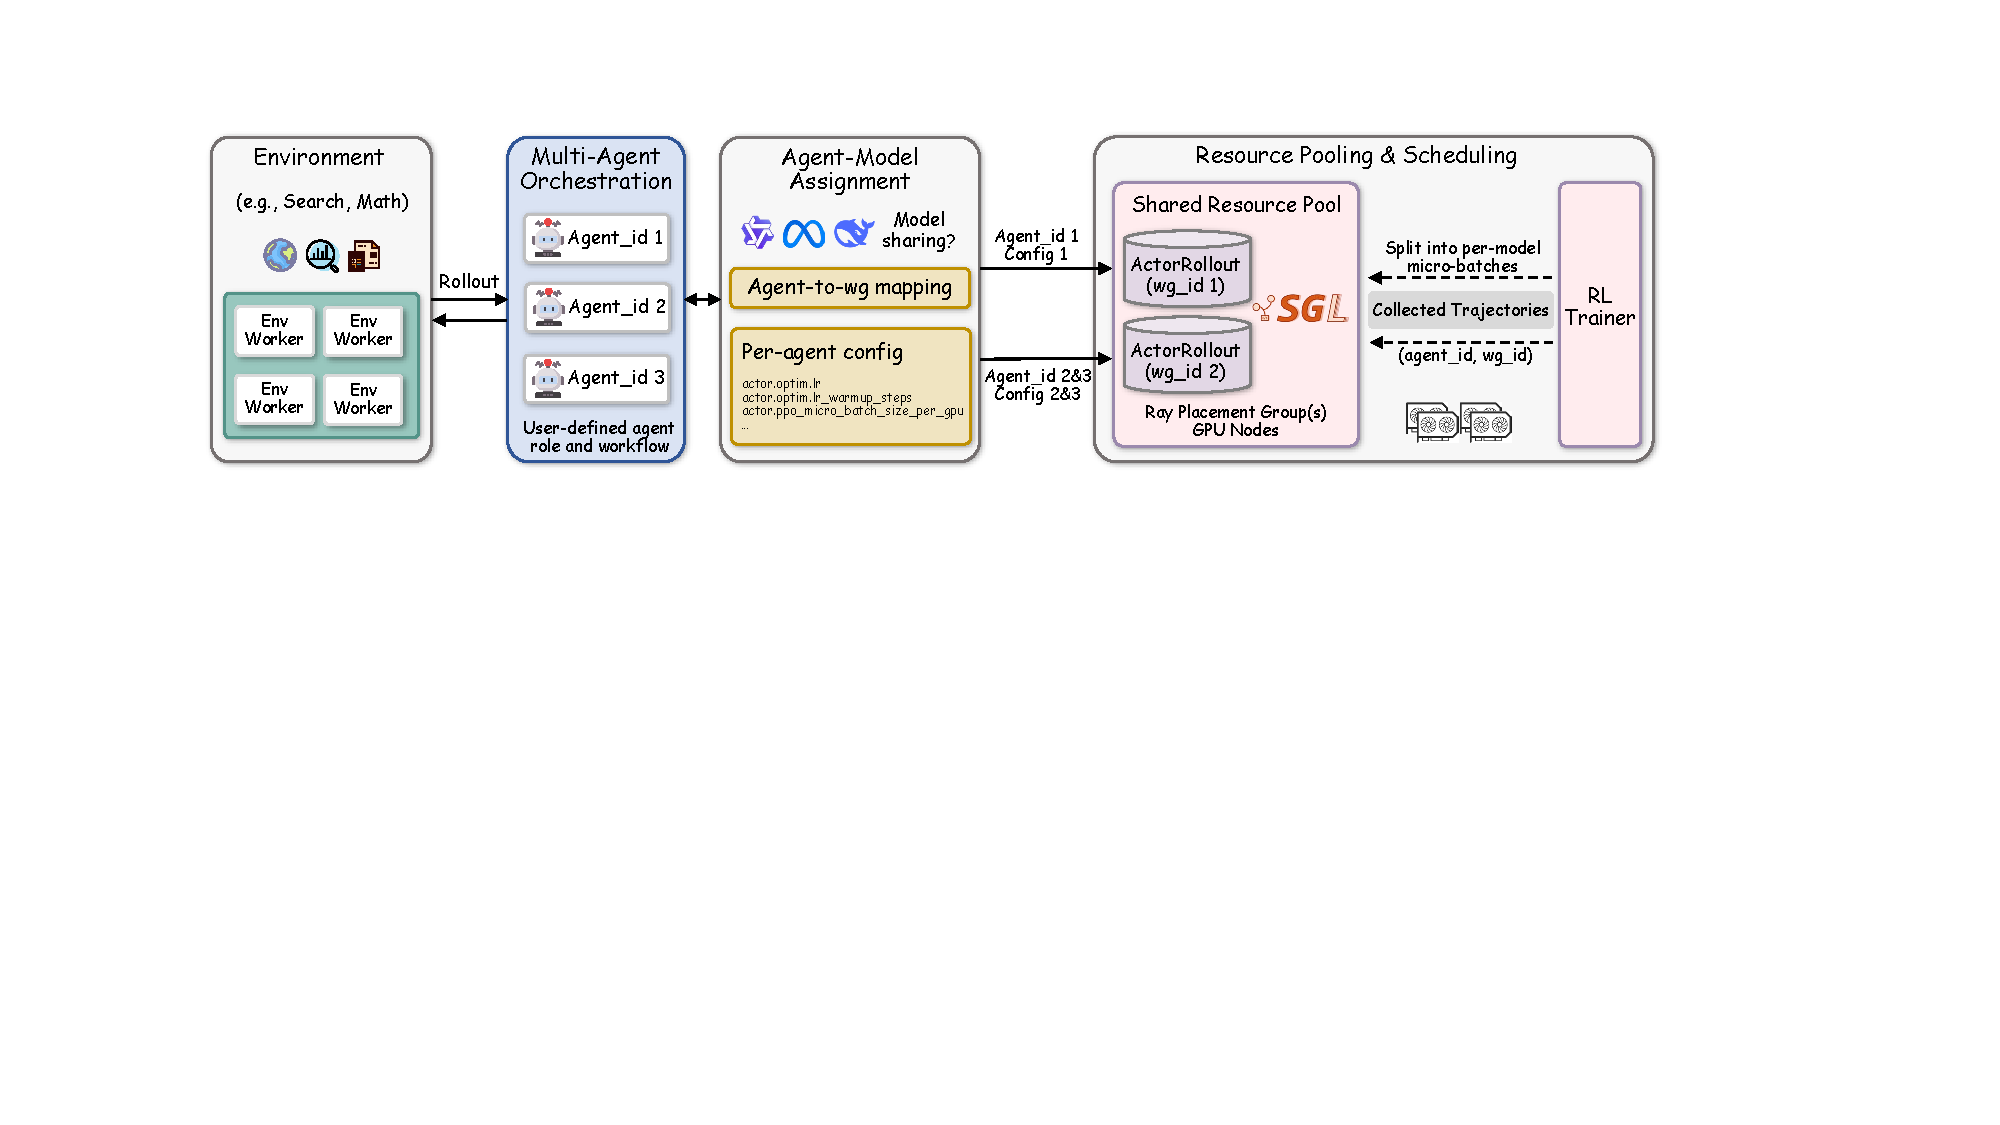
\includegraphics[width=1.0\linewidth]{./figure/drmas_framework.pdf}
   \end{center}
   \vspace{-0.1in}
   \caption{Overview of multi-agent LLM RL framework. A multi-agent orchestrator manages distributed rollouts, agents are mapped to LLM worker groups with optional LLM  sharing, and a shared resource pool schedules actor backends for efficient inference and per-model optimization.}
   \label{fig:framework}
\end{figure*}
\subsection{Framework for Multi-Agent LLM RL}
\label{sec:framework}
We next present a unified system framework that realizes end-to-end RL post-training for multi-agent LLMs. As illustrated in Figure~\ref{fig:framework}, the system is designed to ensure well-conditioned gradient updates across agents, while maintaining scalable orchestration, flexible agent-model assignment, per-agent optimization configs, and efficient hardware utilization for multi-agent rollouts.

\textbf{Multi-Agent Orchestration.}~
Our system is coordinated by a multi-agent trajectory collector, which manages the distributed interaction between the multi-agent LLM system and the environment. It delegates the rollout to a user-defined multi-agent orchestra, which governs the agent roles and execution flow. The orchestra dynamically selects and invokes agent policies based on the current state or prior agent outputs, enabling flexible and conditional control over multi-agent decision-making.

\textbf{Agent-Model Assignment.}~
A core assignment logic maps logical agents ($1,\dots,K$) to physical LLM worker groups (\texttt{wg\_id}). In non-shared settings, each agent $k$ is assigned a distinct worker group (e.g., 7B and 3B models). Conversely, in shared settings, all agents configured with the same model are mapped to a single, shared worker group, allowing joint training and inference while reusing model weights. 

\textbf{Per-Agent Configuration.}~
\methodname{} supports agent-specific training hyperparameters for granular control. This allows configurations like \texttt{actor.optim.lr} to be specified on a per-agent basis. Our system injects the $k$-th hyperparameter set into the configuration for agent $k$, which is then attached to its corresponding LLM work group. A runtime check ensures that all agents sharing the same worker group utilize identical configurations.

\textbf{Shared Resource Pooling and Scheduling.}~
This component decouples logical agent-model assignments from physical resource placement. A resource pool manager provisions hardware resources (e.g., GPUs) into named pools. All LLM actor backends (one for each \texttt{wg\_id}) are mapped to the \texttt{ActorRollout} role. To support high-throughput and low-latency decoding in multi-agent rollouts, these actor backends use \texttt{sglang}~\citep{zheng2024sglang} as the inference engine. This allows them to be co-provisioned within the same shared resource pool using Ray placement groups, enabling scalable scheduling of multiple concurrent LLMs. Agent calls are routed by an \texttt{agent\_to\_wg\_mapping} ($\texttt{agent\_id} \rightarrow \texttt{wg\_id}$). This mapping dynamically dispatches the agent's generation request to the correct backend worker group (\texttt{actor\_rollout\_wg[wg\_id]}).
In the optimization phase, the trainer partitions the aggregated batch $\mathcal{B}$ into per-model micro-batches ${\mathcal{B}_{\text{wg}}}$ according to their worker group ID. Policy updates are then performed for each worker group, ensuring that gradients from an agent's trajectories only update its designated LLM backend.